\section{Evaluation}
\label{sec:eval}

% These top level graphs are based on raw data and pick some select points.
% If you want to see the full tput-latency graphs, uncomment the section of graphs at the bottom

%%%%%%%%%%%%%%%%%%%%%%%%%%%%%%%%%%%%%%%%
%%%%%%%%%%%% Uniform fanout %%%%%%%%%%%%
%%%%%%%%%%%%%%%%%%%%%%%%%%%%%%%%%%%%%%%%
\begin{comment}
% Single shard p99 + p50
\begin{figure*}[!htb]
\centering
\subfloat[1 shard p99]{
  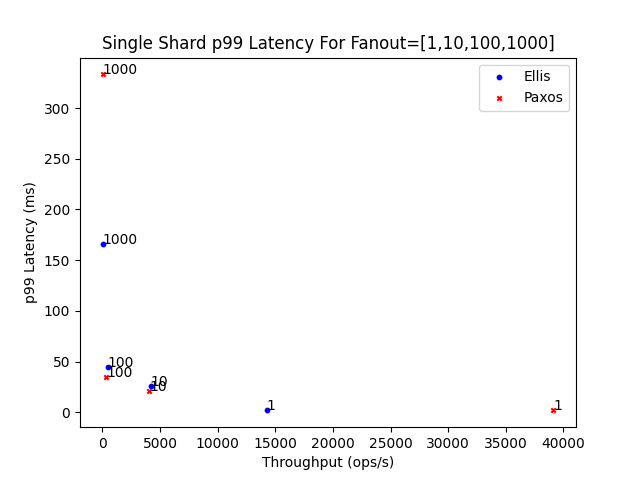
\includegraphics[scale=.6]{figs/1shardp99.png}
  \label{fig:1shardp99}
}
\subfloat[1 shard p50]{
  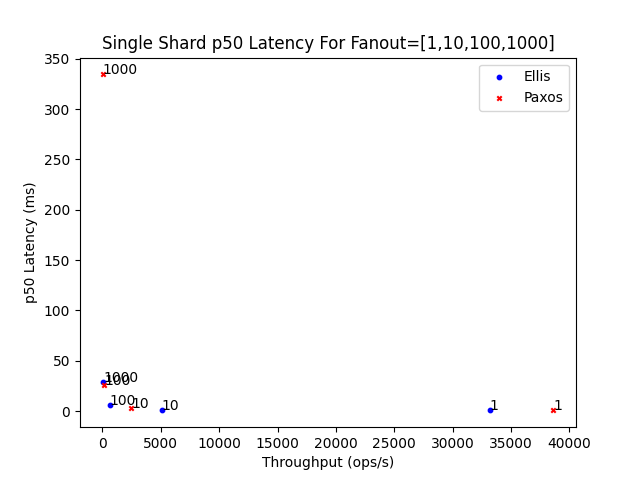
\includegraphics[scale=.6]{figs/1shardp50.png}
  \label{fig:1shardp50}
}
\hspace{0mm}
% 3 shards p99 + p50
\centering
\subfloat[3 shard p99]{
  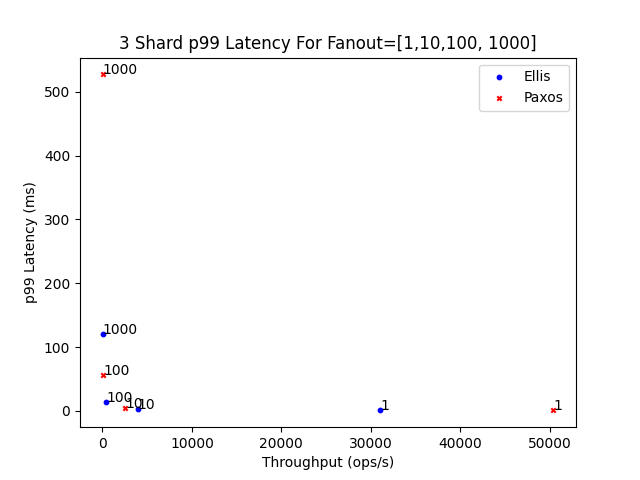
\includegraphics[scale=.6]{figs/3shardp99.png}
  \label{fig:3shardp99}
}
\subfloat[3 shard p50]{
  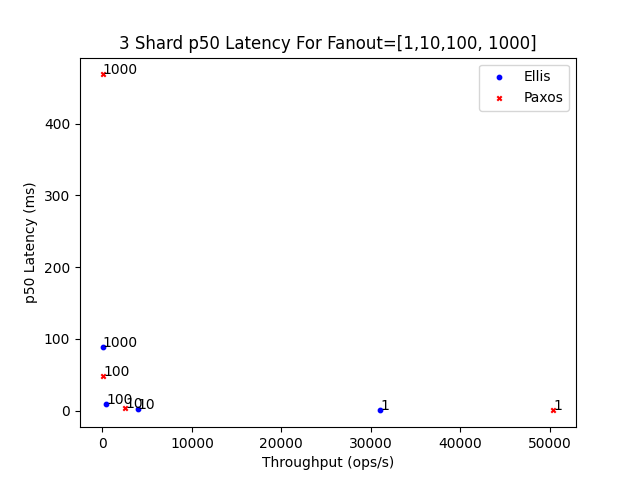
\includegraphics[scale=.6]{figs/3shardp50.png}
  \label{fig:3shardp50}
}
\hspace{0mm}
% 9 shards p99 + p50
\centering
\subfloat[9 shard p99]{
  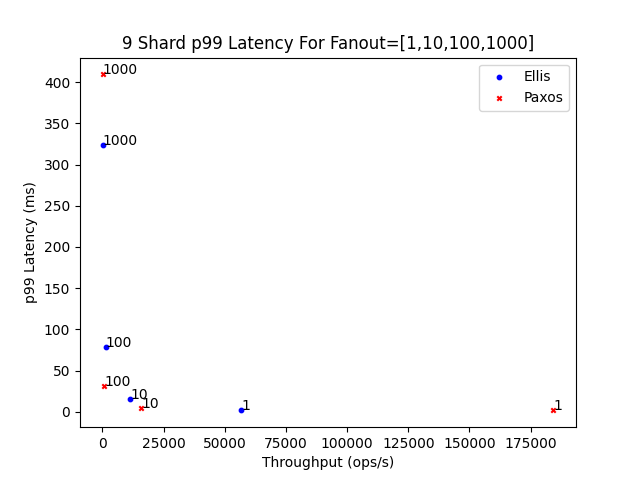
\includegraphics[scale=.6]{figs/9shardp99.png}
  \label{fig:9shardp99}
}
\subfloat[9 shard p50]{
  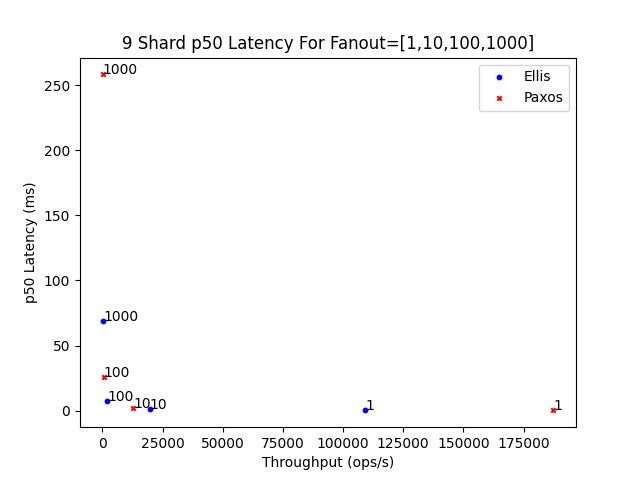
\includegraphics[scale=.6]{figs/9shardp50.png}
  \label{fig:9shardp50}
}
\caption{p99 and p50 for various shard settings.}
\end{figure*}
\end{comment}

We evaluate \sys{}'s performance handling requests from multi-dispatch clients
compared to Multi-Paxos's performance handling requests from single-dispatch
clients.  We focus on measuring the latency of end-to-end
application-level requests that fan out to multiple data store operations.
%We report on both the p99 and p50 for application-request latency.
%We find p50 a useful metric to look at since our decision to evaluate application-level requests is already end-user facing.
This evaluation aims to answer the following questions:
\begin{enumerate}[leftmargin=*]
    \item How does the end-to-end application latency for \sys{} compare to Multi-Paxos in a datacenter setting?
    \item How does it compare in a wide-area setting?
    % \item How does the throughput of \sys{} compare to Multi-Paxos, and how is that affected by batching?
    % \item How sensitive is the performance to skewed workloads?
    % \item \todo{Don't work on this yet, we'll almost certainly have to cut it for space.} What is the effect of the first-operation optimization on latency and throughput in a single-shard setting?
\end{enumerate}

% \stale{We show \sys{} has lower throughput than Multi-Paxos for any particular
% number of shards but reduces end-to-end latency for application-level requests
% by up to 75\% when fanout increases and scales with the number of shards. Moreover, we show that \sys{} significantly outperforms Multi-Paxos in a variety of wide-area configurations.}

\subsection{Experimental Setup}
All experiments ran on Cloudlab's Utah platform, using
m510 machines~\cite{duplyakin2019cloudlab}.  Each machine has 1 Intel Xeon-D processor with 8 physical cores
running at 2 GHz (hyper-threading enabled), 64 GB of DDR4-2133 RAM, and a 10
Gb/s NIC\@.  Our setup consists of a 9-node server cluster and 8 additional client machines.
The round-trip latency between all machines is 150--200 $\mu$s.  Each shard has three replicas,
on different physical machines. For multi-sharded experiments we place
shard leaders on separate physical machines. Clients are distributed
evenly across the client machines.

\wl{@anja delete this after reading: the use of texttt I find to be distracting. and when it's printed out by some readers (like me at home) it looks terrible interspersed with regular text so I'm eliminating it.}

% We do not consider failures in this evaluation. Failures degrade performance for
% most protocols but are rare. Thus, \emph{performance} under failures is not a goal
% for either \mpaxos{} or \system{}. Section~\ref{sec:design} describes how \system{}
% handles failures.
% \wl{We can probably cut the preceding paragraph, and if we keep it this is not the right place for it. We should instead talk about it abbove in 7.0 where we talk about we do evaluate too.}


% \al{combine experimental set-up and client design. get rid of metrics, workload,
% failures and replace with, approximately, one sentence each in the experimental
% setup or eval intro}

%\subsection{Client Design}
Clients submit application-level requests. Each application-level request
submits $n$ (the fanout parameter for an experiment) system-level operations.

Single-dispatch clients interacting with \mpaxos{} have one in-flight operation at
a time. Multi-dispatch clients interacting with \system{} send $n$ system-level
operations concurrently, in order, waiting until all operations complete before
issuing the next batch. Both are closed-loop clients that submit a single
application-level request at a time.
In each experiment, we scale the number of clients issuing requests to both
systems to explore points of low load up through saturation.
%, including from 2 to 8192 clients.by.

% \al{idk... is it worth noting? If so, not here}
% It's worth noting that since multi-dispatch clients have $n$ requests in-flight at a time, while single-dispatch clients only have 1 request in-flight at a time, \system leaders have to deal with $n$ more requests than \mpaxos at any given time for the same number of clients.

%For a fair comparison between MDL and SDL, we keep the number of outstanding requests sent to each system the same. To achieve this, MDL uses a smaller number of clients $K$ with the specified number $N$ of outstanding requests per client, while SDL uses $K*N$ clients each with 1 outstanding request per client.

% \wl{How does keeping the overall number of requests the same mean the load is the same? We discussed this, you can explain this clearly: keep number of outstanding requests the same in both systems, for mdl this uses a smaller number of clients with the specified number of outstanding requests per client, for sdl its N clients with 1 outstanding request per client.}

%\subsection{Workload}
%We consider uniform and skewed key distributions to explore a more representative range of realistic workloads. For the latter, we generate keys according to a Zipfian distribution with varying skew values $\theta \in \{0.5, 0.7, 0.9, 1.1, 1.3\}$, and use a keyspace of size 1 million.
%
%We do not vary the request type at all, all workloads are 100\% writes, since neither our protocol nor basic Paxos implement op-type specific optimizations.


\subsection{Latency in a Single Datacenter}
\label{sec:shards}
%%%%%%%%%%%%%%%%%%%%%%%%%%%%%%%%%%%%%%%%%%%%%%%%%%%%%%%%%%%%%%%%%%%%%%%%%%%%%%%%%%%
%%%%%%%%%%%%%%%%%%%%%%%%%%%%%%%%%%%%%%%%%%%%%%%%%%%%%%%%%%%%%%%%%%%%%%%%%%%%%%%%%%%
%%%%%%%%%%%%%%%%%%%%%%%%%%%%%%%%%%%%%%%%
%%%%%%%% 1 shard uniform p99 %%%%%%%%%%%
%%%%%%%%%%%%%%%%%%%%%%%%%%%%%%%%%%%%%%%%
\begin{figure}[tbp]
\centering
  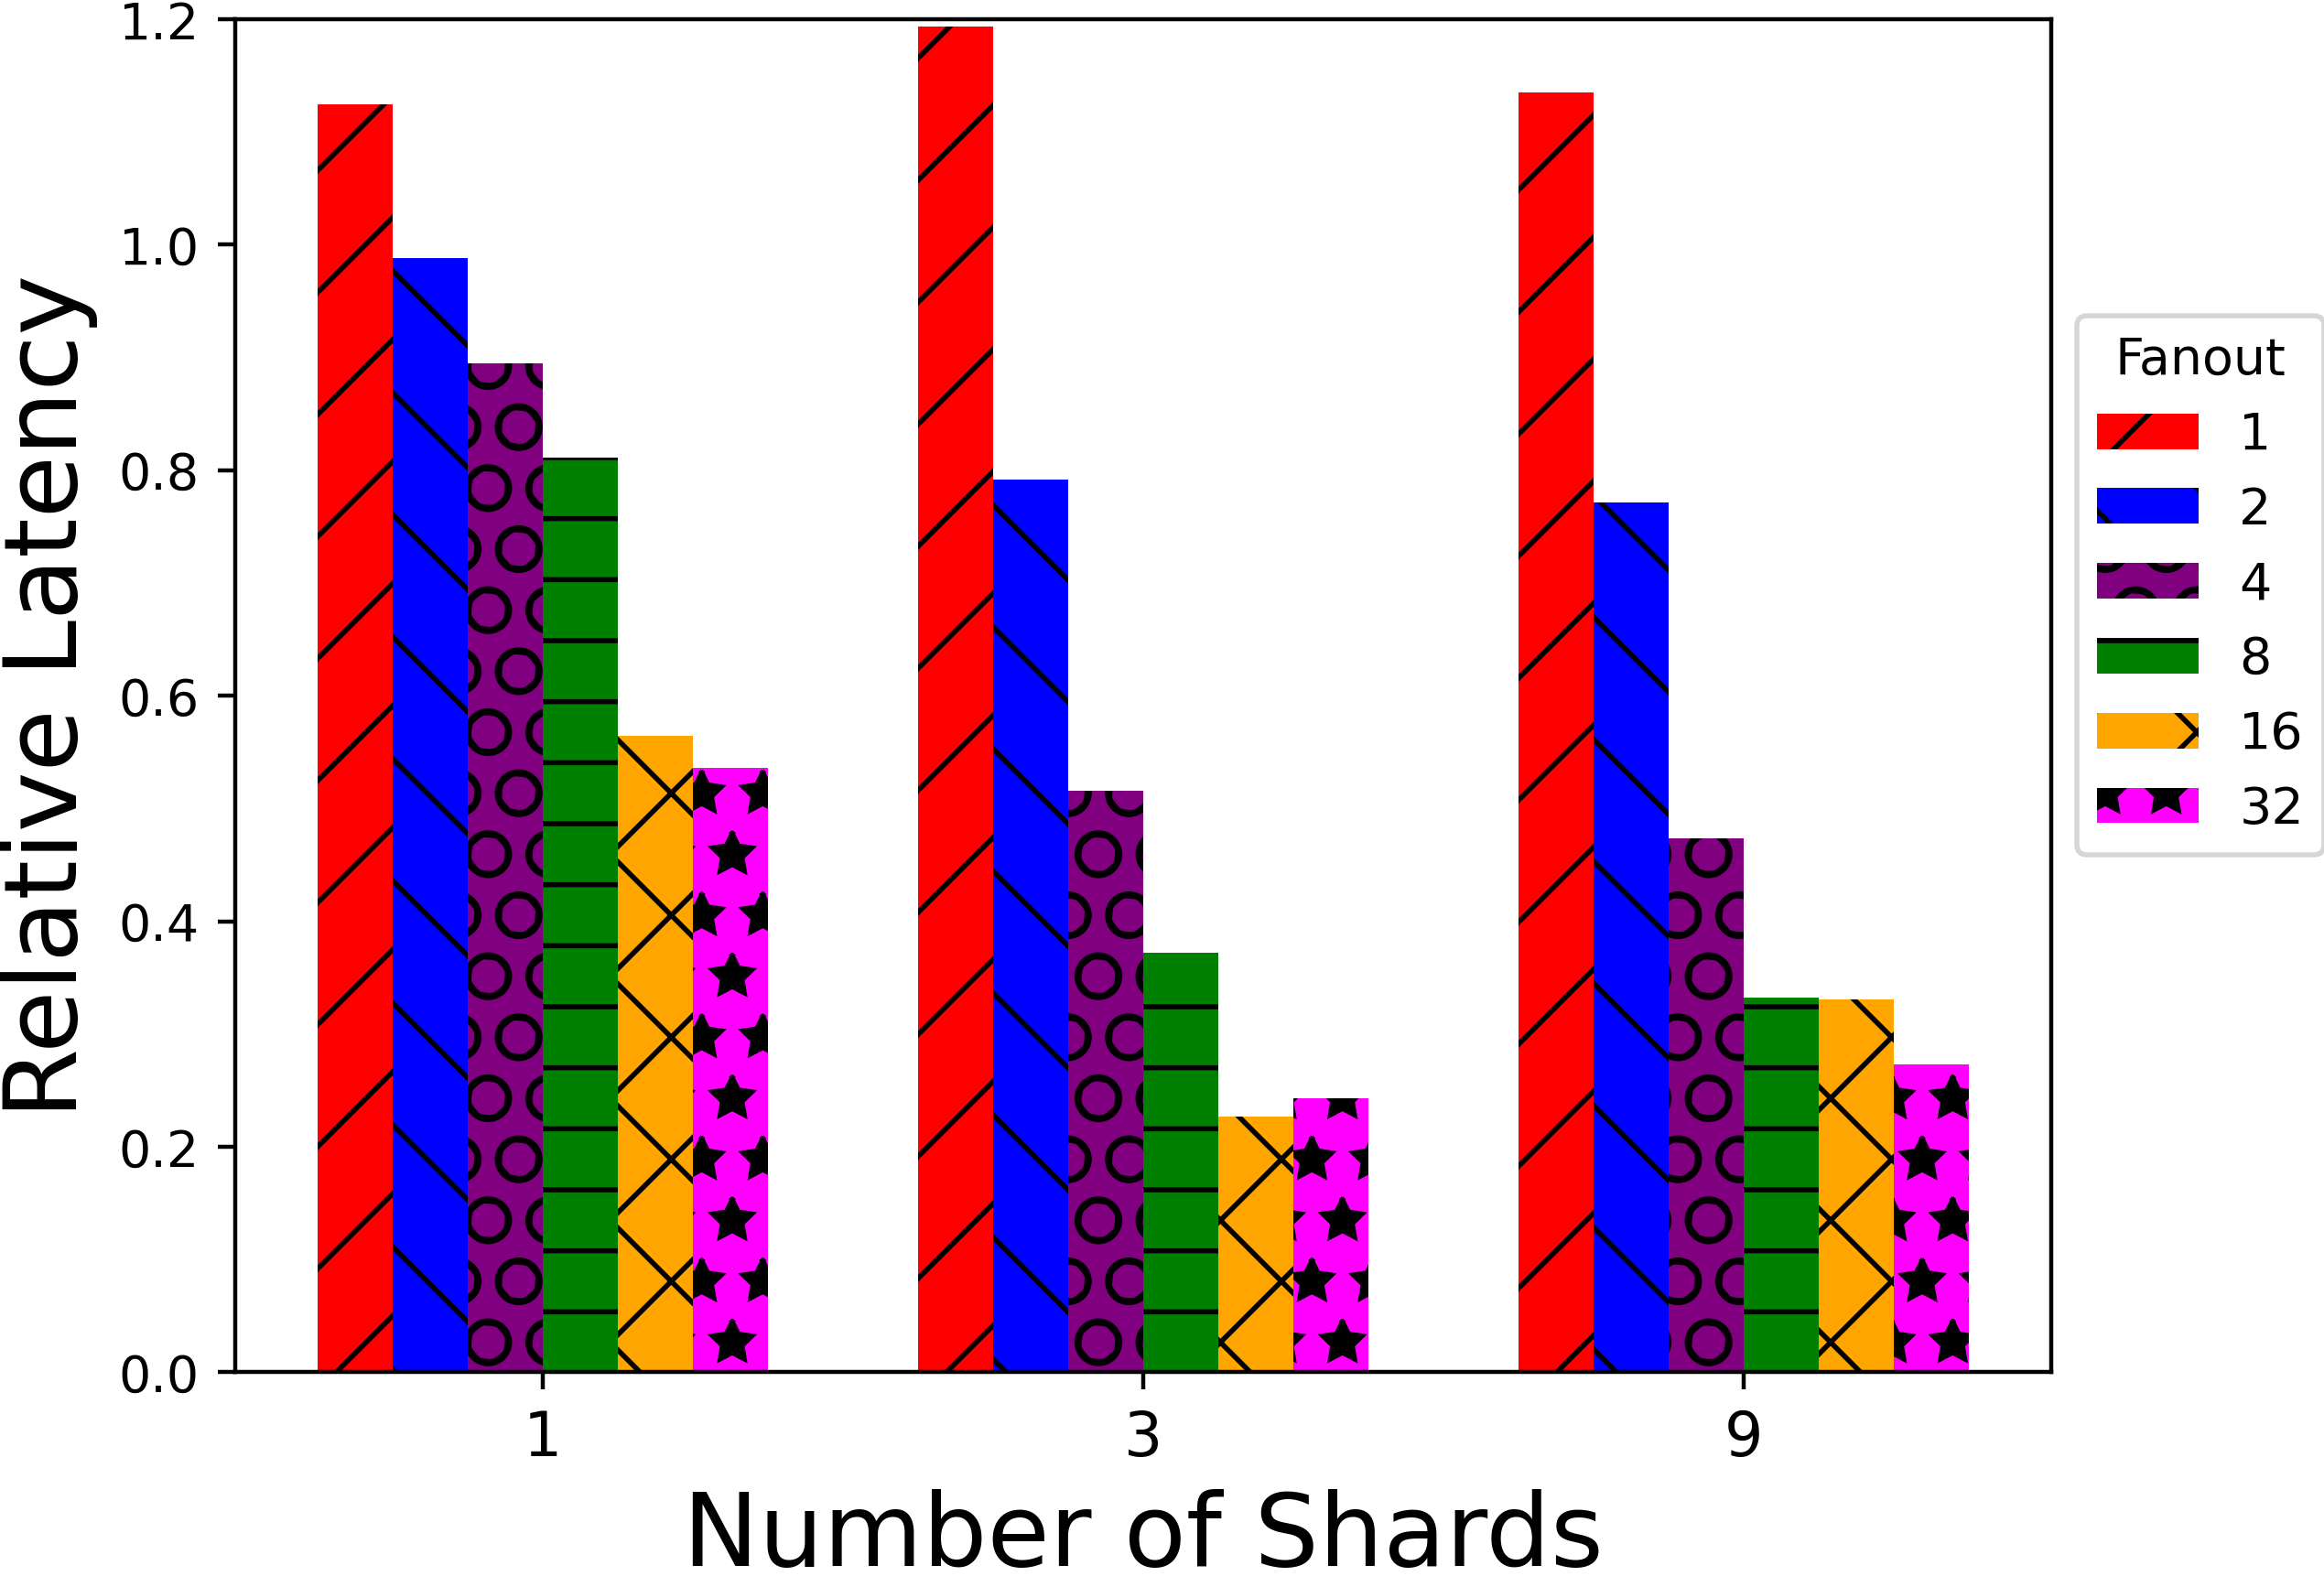
\includegraphics[width=\linewidth]{figs/singleDC.png}
  \vspace{3pt}
\caption{Normalized p50 latency in a single datacenter setting with 1, 3, and 9 shards for fanouts of 1--32. Latency for each setting is normalized to the \mpaxos{} latency.}
%p99 latency for a single datacenter setting. We show results for a sweep of fanouts on 1 shard, 3 shards, and 9 shard clusters.}
\label{fig:DC}
\end{figure}
%%%%%%%%%%%%%%%%%%%%%%%%%%%%%%%%%%%%%%%%%%%%%%%%%%%%%%%%%%%%%%%%%%%%%%%%%%%%%%%%%%%
%%%%%%%%%%%%%%%%%%%%%%%%%%%%%%%%%%%%%%%%%%%%%%%%%%%%%%%%%%%%%%%%%%%%%%%%%%%%%%%%%%%

Figure~\ref{fig:DC} compares the median
end-to-end application request latency for \system{} and \mpaxos{}
configured in a single datacenter with a uniform key distribution and fanouts from $1$ to $32$. We show latencies for single- and multi-shard settings.

At a fanout of 1, the latency of application-level requests is roughly the same between \system{} and \mpaxos{}, since the first request in a set of concurrent requests issued to \system{} only requires a single round. We expect to see significant latency improvements as the fanout increases, approaching an upper bound of 1/4 as discussed in \Cref{sec:design}.

In the single shard setting, we do not reach the upper bound due to inefficiencies in our implementation, which is not optimized for the single shard case.
% In a single shard setting, the upper bound cannot be reached due to several reasons. In particular, when the leader is under high load at higher
% fanouts, it must process a large log of buffered
% requests and each of their coordination messages. The protocol evaluated is not optimized for a single shard, so coordination messages are still issued even though the recipient and sender is the same. Lower latency is attenuated by the processing of coordination overhead
% for each request. While not shown, this improvement is even
% greater for p90 and p50, where the tail variability of subrequest latency is less pronounced.
%
%Somewhat counter-intuitively, three shards outperforms nine. 
As the number of shards increases, however, we notice latency approaches the lower bound improvement
described in \cref{sec:design} for fanouts $8$, $16$, and $32$, with latency
close to 25\% of \mpaxos{}. p90 and p99 latency also approaches 1/4 of \mpaxos{} (not shown).
% An application-level request of fanout $n$ induces
% $n-1$ 1-way inter-shard coordination messages that must be serialized with
% predecessor fault-tolerance and coordination. On the other hand, load balancing
% of large number of requests across multiple shards helps speed the processing
% time at each leader.
%
Overall, \sys{} provides the same latency as \mpaxos{} when there is no potential for parallelization and lower latency when there is potential parallelization at fanouts of 2 or more.

% * Compare e2e app latency in a single datacenter setting\\
% * The latency between clients and shard leader, shard leaders and shard leaders,  and shard leaders and replicas is uniform and low\\

% * Main graph:\\
% * y-axis: latency (yrange starts from 0!)\\
% * x-axis: setting (fanout 1, 2, 8 (or 10), 32)\\
% * bars: show box-and-whiskers plot with (something like) p1, p10, p50, p90, p99 for ellis, and also multi-paxos\\
% * these results should be under relatively moderate load, i.e., choose the highest throughput where both systems still have pretty flat latency (so we aren't see throughput/queuing effects)\\
% * (This looks like the COPS graph I sent you on slack)\\

% * Interpret results \ main takeaway\\
% * fanout 1 is the same because of the optimization\\
% * fanout 2 we have a little bit lower latency, explain\\
% * fanout 10, 32 we have much lower latency, explain\\

% * overall conclusion:\\
% * latency is always the same when there is no potential parallelization (fanout 1) or lower when there is potential parallelization (fanout 2 or more)\\
% * as fanout increases the latency win approachs 3/4\\


\begin{table}[b]
\begin{tabular}{@{}lrrr@{}}
& \multicolumn{3}{c}{Latencies}  \\
& C $\leftrightarrow$ SL & SL $\leftrightarrow$ SL & SL $\leftrightarrow$ R  \\
Edge Client  & 90\,ms  & 2\,ms & 90\,ms  \\
%Colocated Shards/Clients & 2\,ms  & 2\,ms & 90\,ms  \\
Datacenter Clients    & 2\,ms & 90\,ms & 90\,ms 
\end{tabular}
\vspace{4pt}
\caption{Latencies between Clients \textit{C}, Shard Leaders \textit{SL}, and Replicas \textit{R} for each of the wide-area configurations investigated.}
\label{table:wan}
\end{table}

\subsection{Latency in the Wide Area}
% * Compare e2e app latency in a wide-area setting\\
% * The latency between clients and shard leader, shard leaders to shard leaders, and shard leaders and replicas is heterogenous and can be high depending on the setting\\
% ** we have 3 settings:\\
% ** ...

% * Main graph (one for each setting):\\
% * y-axis: latency (yrange starts from 0!\\
% * x-axis: setting (fanout 1, 2, 8 (or 10), 32)\\
% * bars: show box-and-whiskers plot with (something like) p1, p10, p50, p90, p99 for ellis, and also multi-paxos\\
% * these results should be under relatively moderate load, i.e., choose the highest throughput where both systems still have pretty flat latency (so we aren't see throughput/queuing effects)\\
% * (This looks like the COPS graph I sent you on slack)\\

% * Interpret results \ main takeaway\\
% * do for each setting in turn\\

% * overall conclusion:\\
% * ... \stale{latency is always the same when there is no potential parallelization (fanout 1) or lower when there is potential parallelization (fanout 2 or more)}\\
% * as fanout increases the latency win approaches (shard\_leader -> shard\_leader)/(client->shar\_leader->replica->shard\_leader->client)\\

%We show the results from running \sys{} in the wide area compared with Multi-Paxos in the wide area.
We compare \sys{} to \mpaxos{} for two wide-area configurations with three shards.
%, representative of real world topologies, that show the limits and benefits of using multi-dispatch over Multi-Paxos.
\Cref{table:wan} shows the specifics of the topologies for each of the 2 configurations. We select a wide-area delay of 90\,ms between datacenters and an intra-datacenter latency of 2\,ms. Both of these values are representative of real-world values and provide enough contrast to highlight differences in performance~\cite{wanpings}.

Overall, \Cref{fig:wan} shows that \sys{} is a good choice for the wide-area, since it can parallelize large latencies present in various toplogies. 




\paragraph{Edge Client.}
In this configuration, clients are far from shard leaders to represent when application-level requests are issued from applications running on client edge devices, which is representative of how many applications run today. In addition, we colocate shard leaders which significantly reduces the coordination overhead present in \sys{}.

As seen in \cref{fig:wan}, single-dispatch suffers from having to sequentially pay for the large latency between edge clients and the backend. Moreover, with minimal coordination overhead for \sys{}, the latency of multi-dispatch exceeds the 1/4 limit that exists when latencies are homogeneous.
% \begin{figure*}[tbp]
% \centering
% \subfloat[fanout\xspace1]{
%   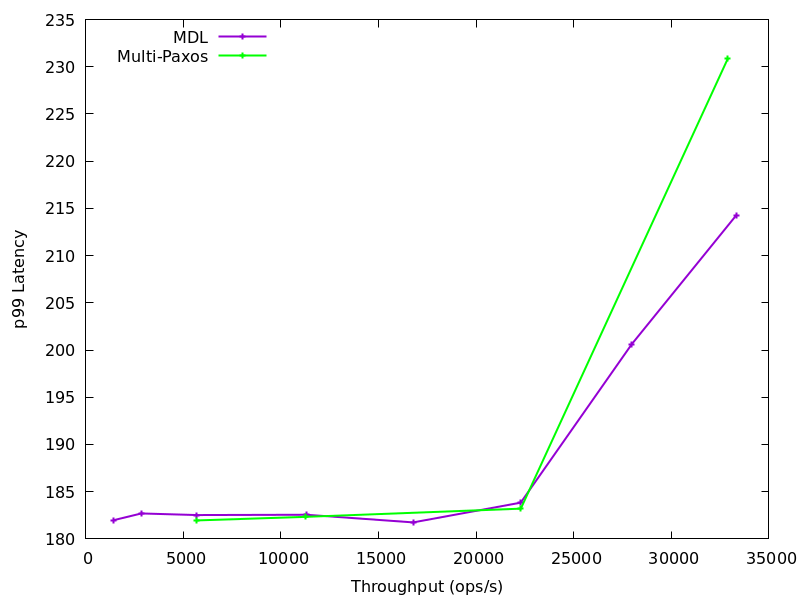
\includegraphics[scale=.17]{figs/wan/wide1/wide1-f1.png}
%   \label{fig:w1f1}
% }
% \subfloat[fanout\xspace2]{
%   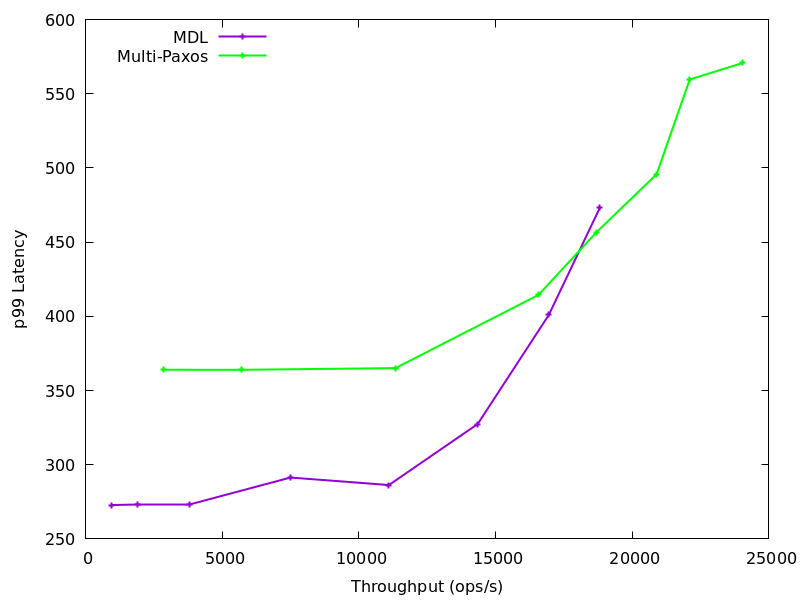
\includegraphics[scale=.17]{figs/wan/wide1/wide1-f2.png}
% }
% \subfloat[fanout\xspace10]{
%   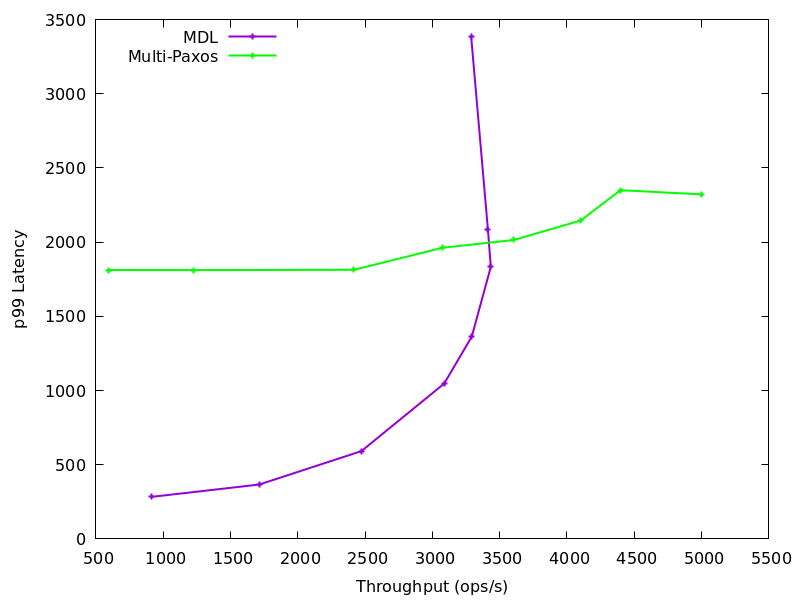
\includegraphics[scale=.17]{figs/wan/wide1/wide1-f10.png}
% }
% \subfloat[fanout\xspace32]{
%   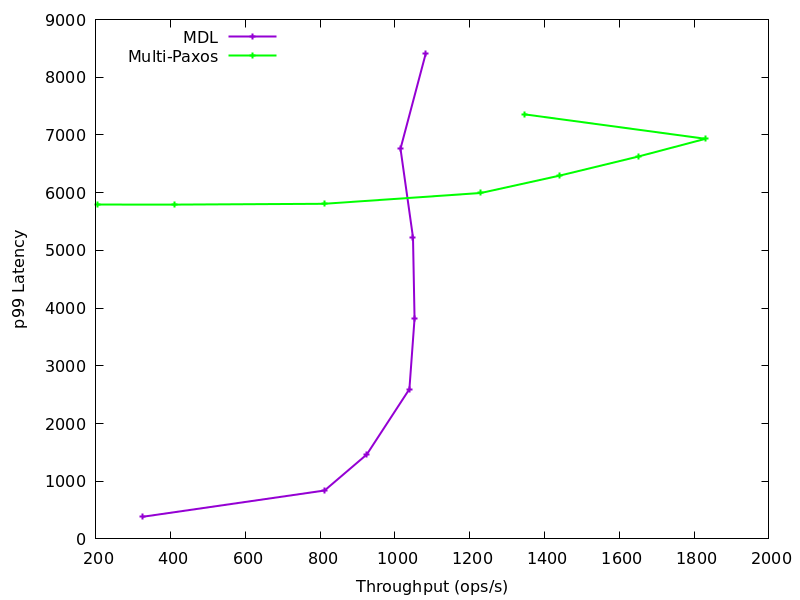
\includegraphics[scale=.17]{figs/wan/wide1/wide1-f32.png}
% }
% \caption{Edge Client WAN results}

% \label{fig:wan1}
% \end{figure*}
\begin{figure}[tbp]
\centering
  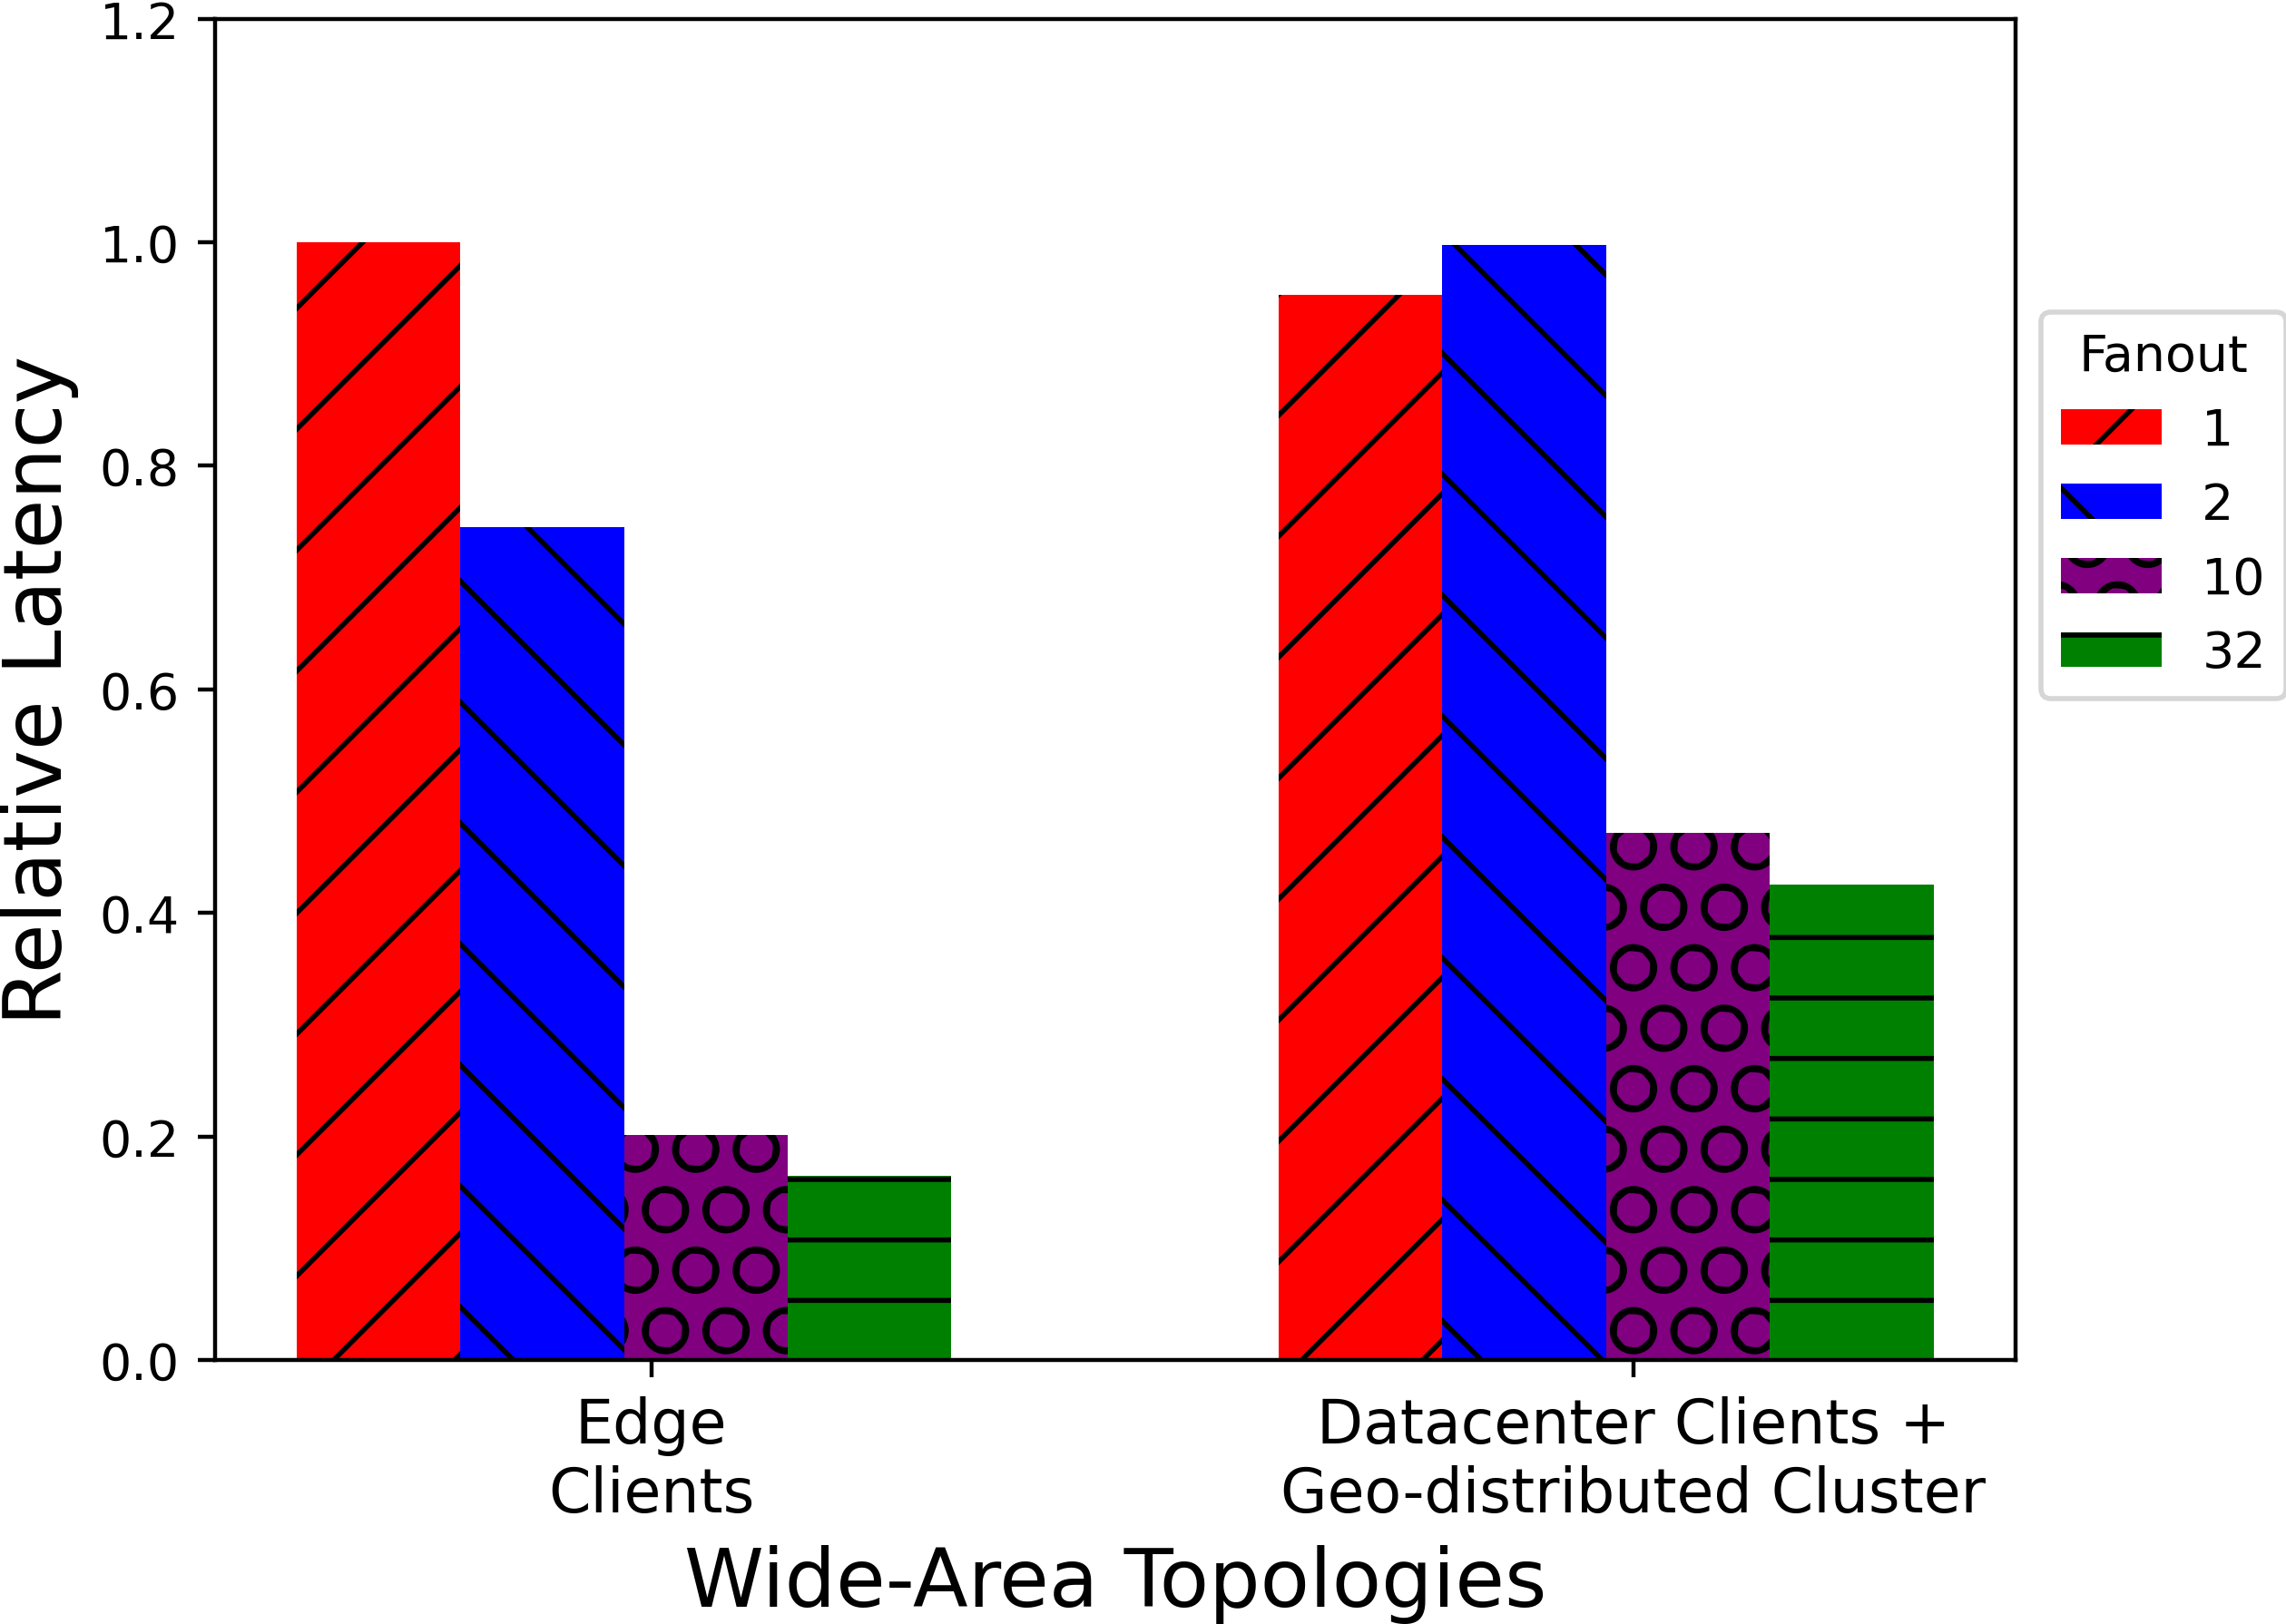
\includegraphics[width=\columnwidth]{figs/wide_area_latencies.png}
  \vspace{1pt}
\caption{Normalized p50 latency in the two wide-area settings with three shards for fanouts of 1--32. Latency for each setting is normalized to the \mpaxos{} latency.}
\label{fig:wan}
\end{figure}

% \paragraph{Colocated Shards and Clients.}
% \todo{Probably going to cut this ... doesn't show much new.}
% In this configuration, clients are in the datacenter and shard leaders remain colocated, to represent geo-replicated settings that benefit from having nearby clients.
% As shown in \Cref{fig:wan}, he perfomrances of the two baselines are similar. Since clients are colocated with shard leaders, single-issue is not the most expensive overhead compared to replication. Moreover, since \sys{} has to pay for two replication rounds between leaders and far away replicas, at high fanouts most of the performance wins are lost.


% \begin{figure*}[tbp]
% \centering
% \subfloat[fanout\xspace1]{
%   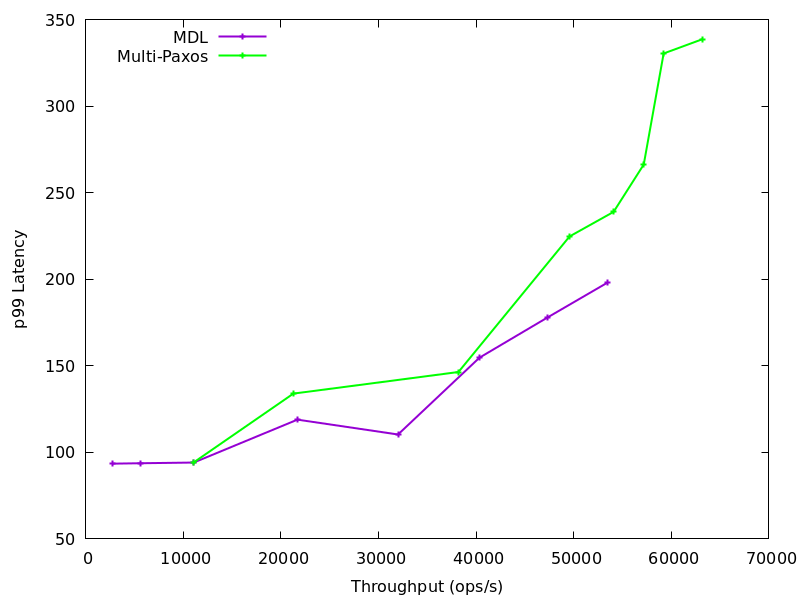
\includegraphics[scale=.18]{figs/wan/wide2/wide2-f1.png}
%   \label{fig:w2f1}
% }
% \subfloat[fanout\xspace2]{
%   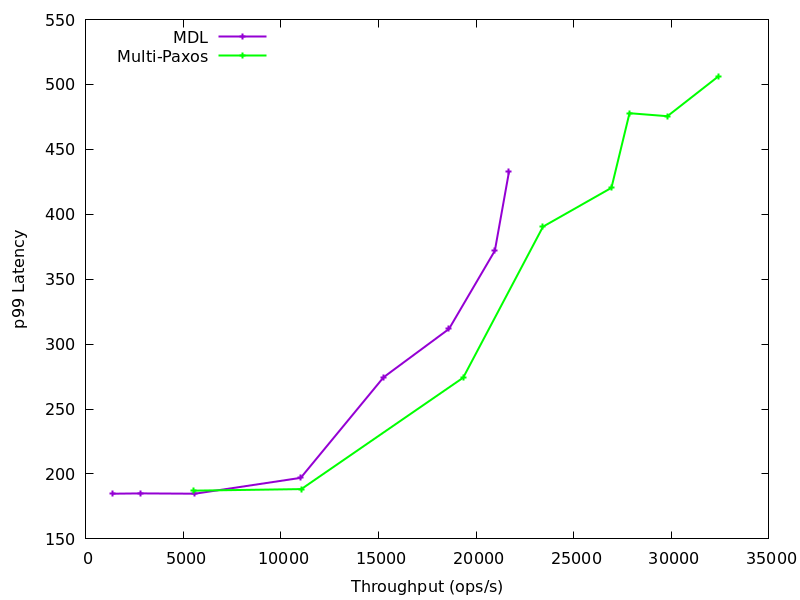
\includegraphics[scale=.18]{figs/wan/wide2/wide2-f2.png}
% }
% \subfloat[fanout\xspace10]{
%   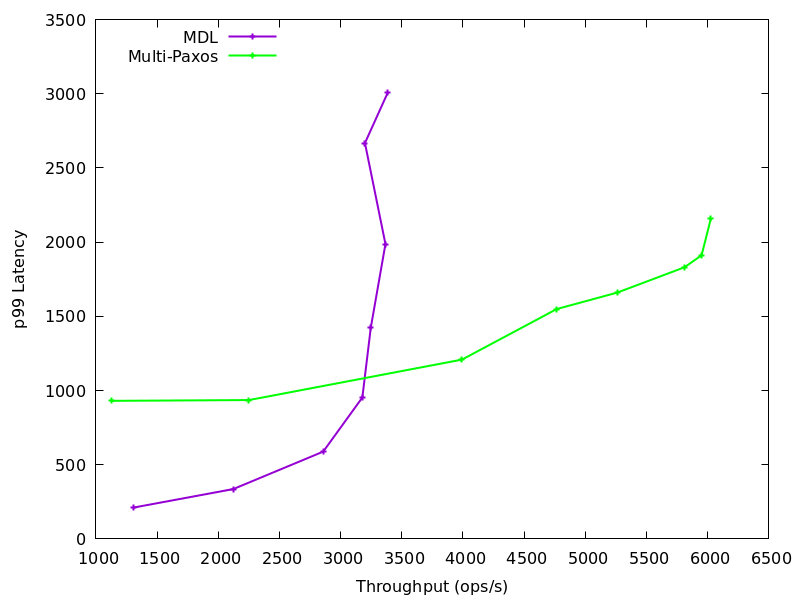
\includegraphics[scale=.18]{figs/wan/wide2/wide2-f10.png}
% }
% \subfloat[fanout\xspace32]{
%   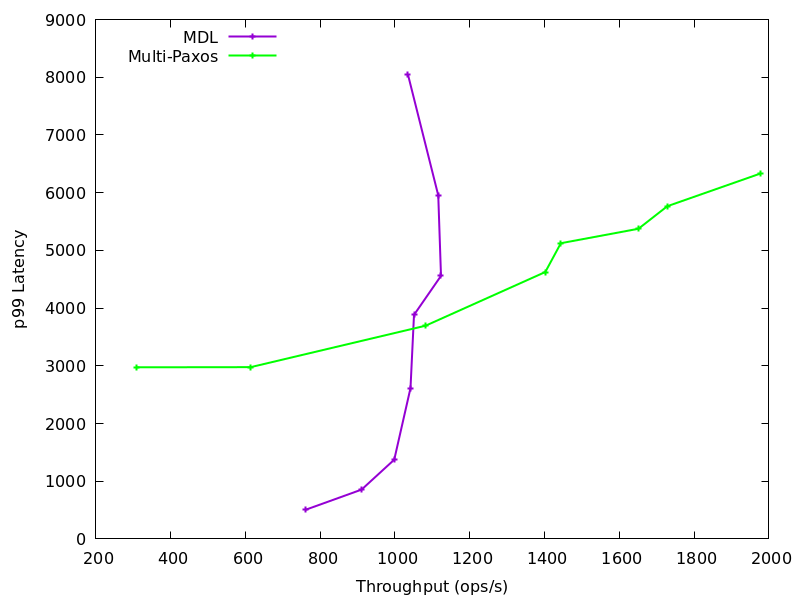
\includegraphics[scale=.18]{figs/wan/wide2/wide2-f32.png}
% }
% \caption{Colocated Shards+Clients WAN results}
% \label{fig:wan2}
% \end{figure*}

\paragraph{Datacenter Clients and Geo-distributed Clusters.}
In this configuration, we inspect the end-to-end performance of clients located in the datacenter, which is realistic for infrastructure applications that would benefit from the usage of multi-dispatch. Moreover, the shard leaders are not colocated, they are also geo-distributed representing the worst case coordination overhead for \sys{}. We show this configuration to display the limitations of \sys{}, making it the setting for which the benefits of \sys{} are least pronounced. As shown in \Cref{fig:wan}, the limit to \sys{}'s improvement here is closer to $1/2$ the latency of \mpaxos{}. This is because as fanout increases the latency of \sys{} grows with the shard-leader-to-shard-leader latency over 45\,ms, while the latency of \mpaxos{} grows with shard-leader-to-replica-and-back latency of 90\,ms.

% A real world example of this topology might be something like an application that shards disjoint data between two far away geographic regions, and places clients directly between these regions. Within this topology, the coordination between shards is expensive, but issuing requests from clients to each shard is less expensive. In practice, the difference in these 2 latencies will never be as extreme as that depicted here, at best a client can be equidistant from all shards to maintain a consistently low wide-area latency roundtrip. Because of this, we expect \sys{} to still be a better choice for these configurations in the real world.

% \begin{figure*}[tbp]
% \centering
% \subfloat[fanout\xspace1]{
%   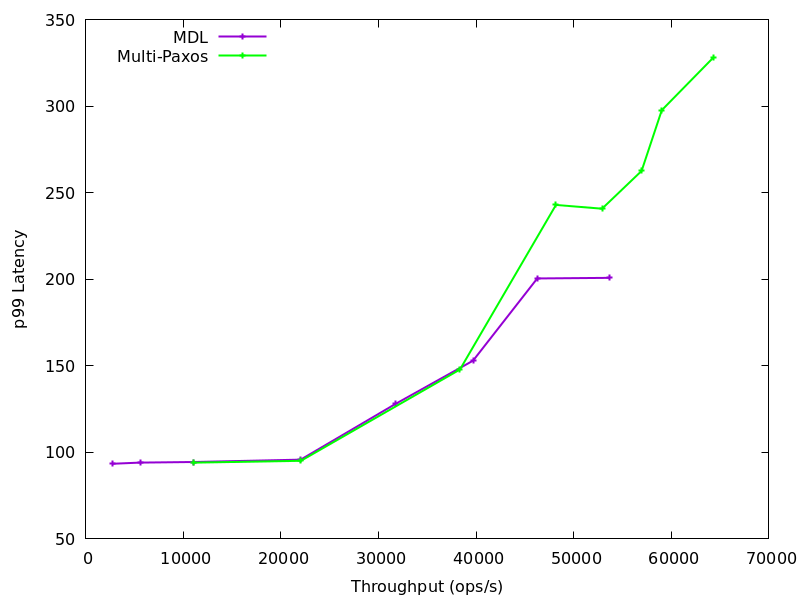
\includegraphics[scale=.18]{figs/wan/wide5/wide5-f1.png}
%   \label{fig:w5f1}
% }
% \subfloat[fanout\xspace2]{
%   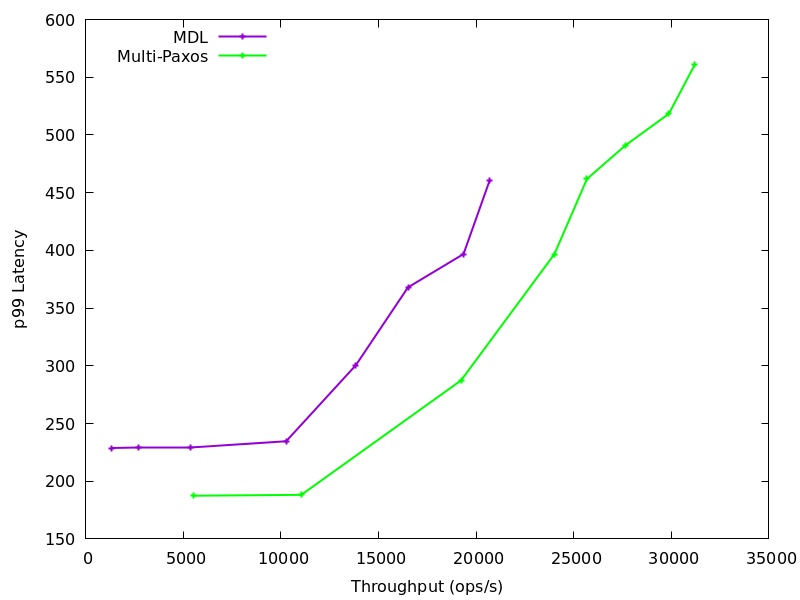
\includegraphics[scale=.18]{figs/wan/wide5/wide5-f2.png}
% }
% \subfloat[fanout\xspace10]{
%   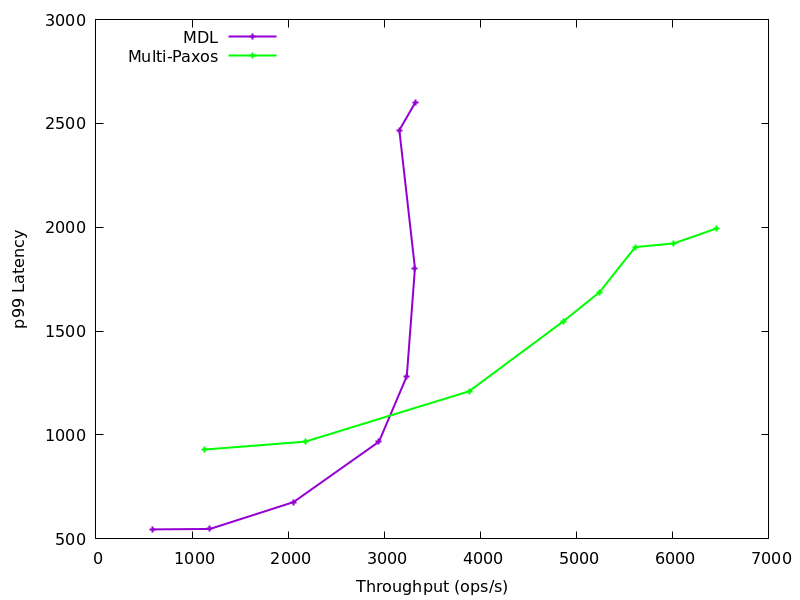
\includegraphics[scale=.18]{figs/wan/wide5/wide5-f10.png}
% }
% \subfloat[fanout\xspace32]{
%   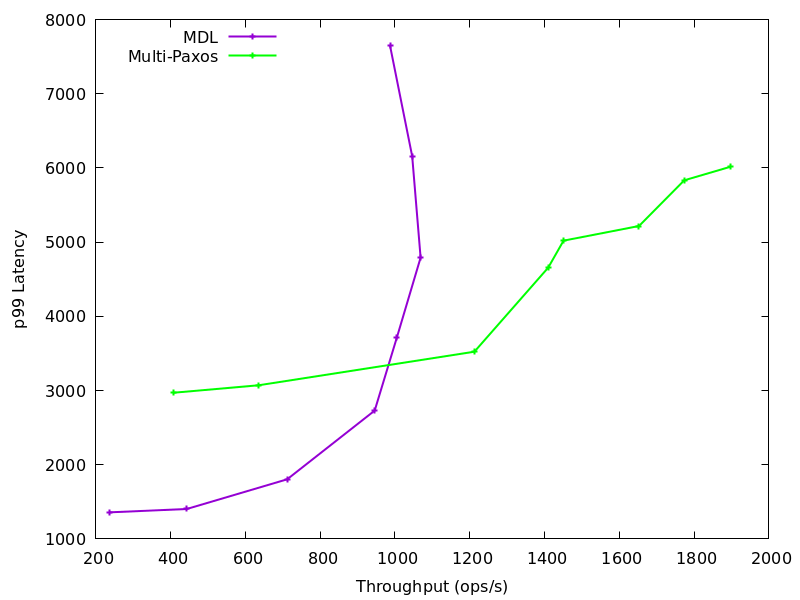
\includegraphics[scale=.18]{figs/wan/wide5/wide5-f32.png}
% }
% \caption{Datacenter Clients WAN results}
% \label{fig:wan5}
% \end{figure*}

% \subsection{Batching}
% We show evaluation for running \sys{} with batching enabled and compare it to Multi-Paxos with batching enabled. We implement batching using timed batching intervals that range from [250us, 500us, 750us, 1ms, 1.5ms, 2ms, 2.5ms, 3ms, 4ms, 5ms, 10ms]. For Multi-Paxos, client requests are collected for the duration of the batching interval, then all of the prepared requests are replicated together. For \sys{}, we apply this usage of batching for both rounds of the protocol, the initial replication round as well as the secondary ordering round, and use the same batching interval duration for both uses.

% Figure ~\ref{fig:batching} shows the results.

% \begin{figure*}[tbp]
% \centering
% \subfloat[mdl\xspace fanout\xspace1]{
%   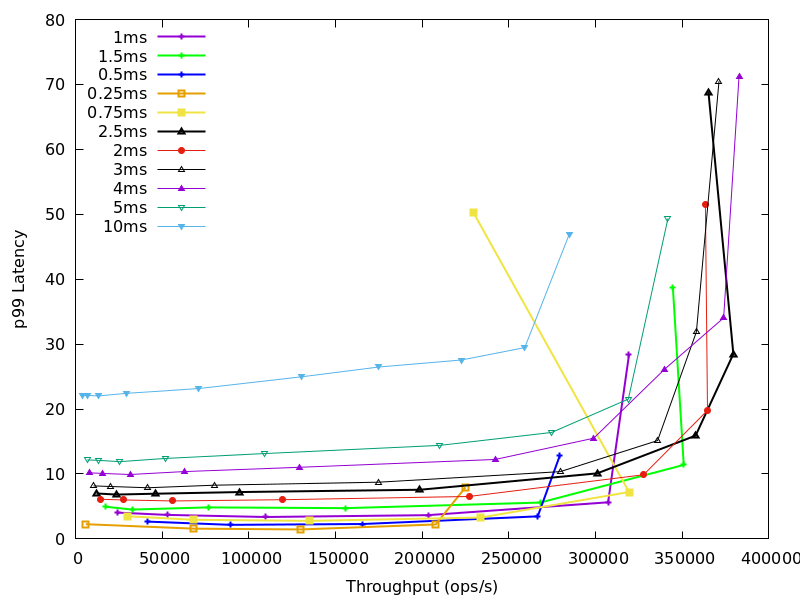
\includegraphics[scale=.2]{figs/batching/mdl_f1.png}
% }
% \subfloat[mp\xspace fanout\xspace1]{
%   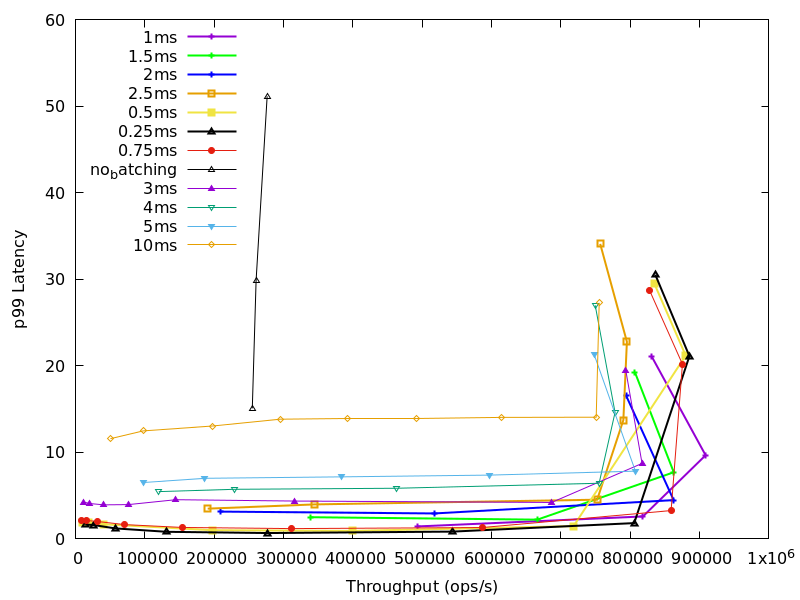
\includegraphics[scale=.2]{figs/batching/mp_f1.png}
% }
% \subfloat[mdl\xspace fanout\xspace10]{
%   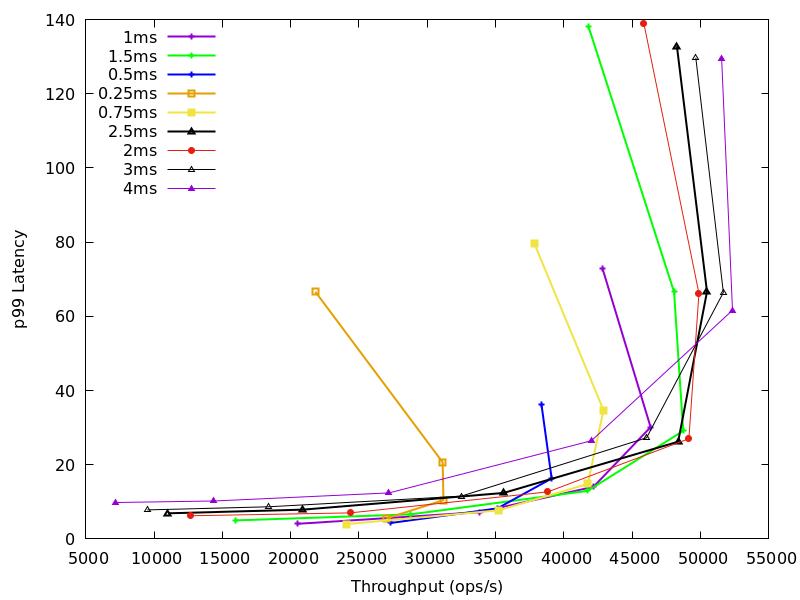
\includegraphics[scale=.2]{figs/batching/mdl_f10.png}
% }

% \subfloat[mp\xspace fanout\xspace10]{
%   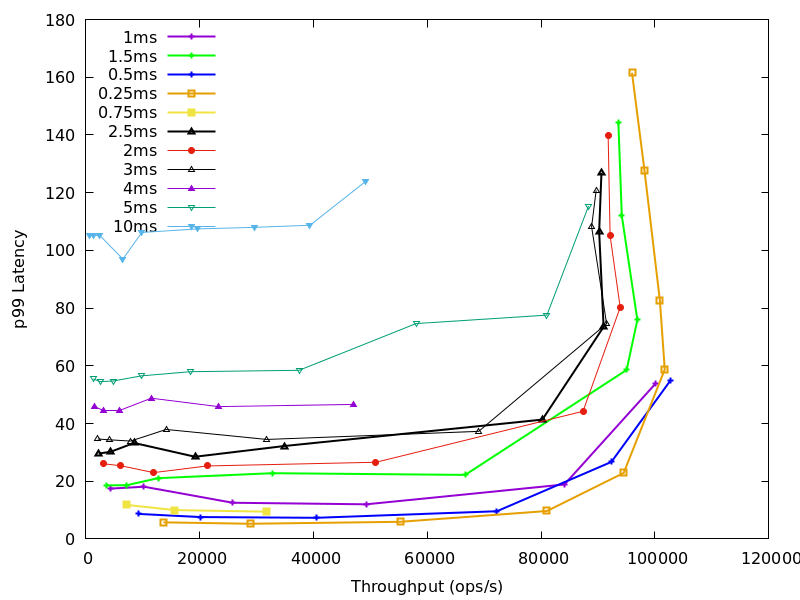
\includegraphics[scale=.2]{figs/batching/mp_f10.png}
% }
% \subfloat[mdl\xspace fanout\xspace100]{
%   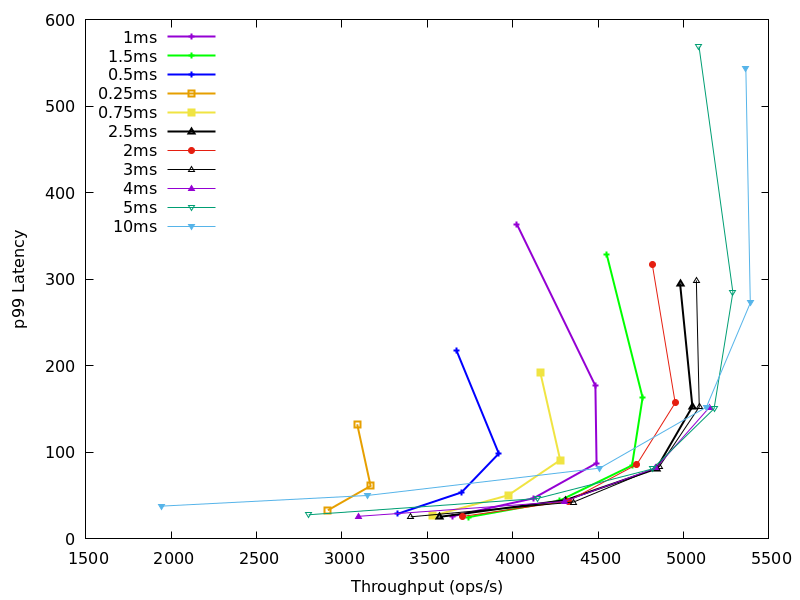
\includegraphics[scale=.2]{figs/batching/mdl_f100.png}
% }
% \caption{Batching Experiments}
% \label{fig:batching}
% \end{figure*}

\subsection{Skew}
Due to space limitations we omit an experimental comparison of \sys{} and \mpaxos{} for varying values of skew. At a high-level we saw that the improvements of \sys{} over \mpaxos{} are robust to varying skew values until we reached a Zipfian value of above 1.1 where overload at a single shard as a result of the extreme skew degrades the improvement.

% %%%%%%%%%%%%%%%%%%%%%%%%%%%%%%%%%%%%%%%%
% %%%%%%%%%%%% 3 shard skew %%%%%%%%%%%%%%
% %%%%%%%%%%%%%%%%%%%%%%%%%%%%%%%%%%%%%%%%
% \begin{figure*}[tbp]
% \centering
% \subfloat[skew\xspace0.5]{
%   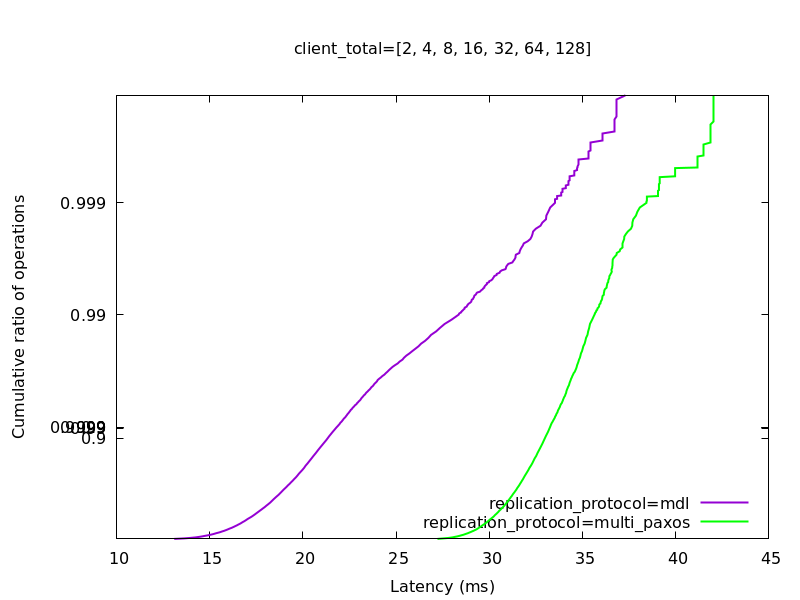
\includegraphics[scale=.2]{figs/3shards_fanout100_skew0.5_8client_CDF.png}
%   \label{fig:3shardsskew}
% }
% \subfloat[skew\xspace0.9]{
%   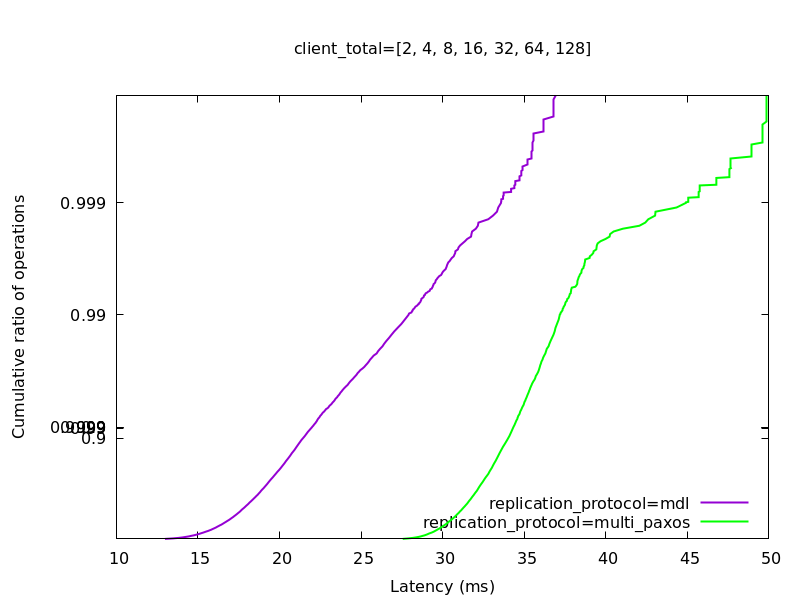
\includegraphics[scale=.2]{figs/3shards_fanout100_skew0.9_8client_CDF.png}
% }
% \subfloat[skew\xspace1.3]{
%   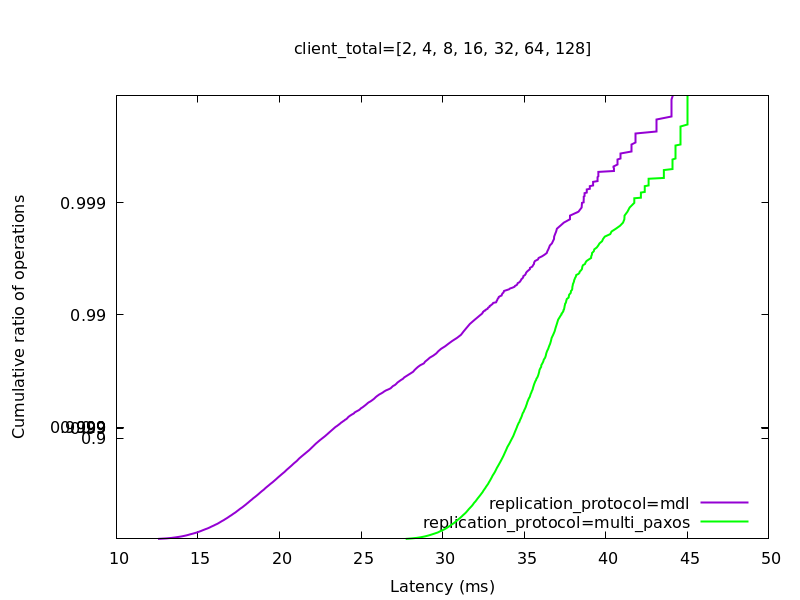
\includegraphics[scale=.2]{figs/3shards_fanout100_skew1.3_8client_CDF.png}
%   \label{fig:3shardsskewlast}
% }
% \caption{3 shard skew.}
% \end{figure*}


%%%%%%%%%%%%%%%%%%%%%%%%%%%%%%%%%%%%%%%%
%%%%%%%%%%%% 9 shard skew %%%%%%%%%%%%%%
%%%%%%%%%%%%%%%%%%%%%%%%%%%%%%%%%%%%%%%%
% \begin{figure*}[tbp]
% \centering
% \subfloat[skew\xspace0.5]{
%   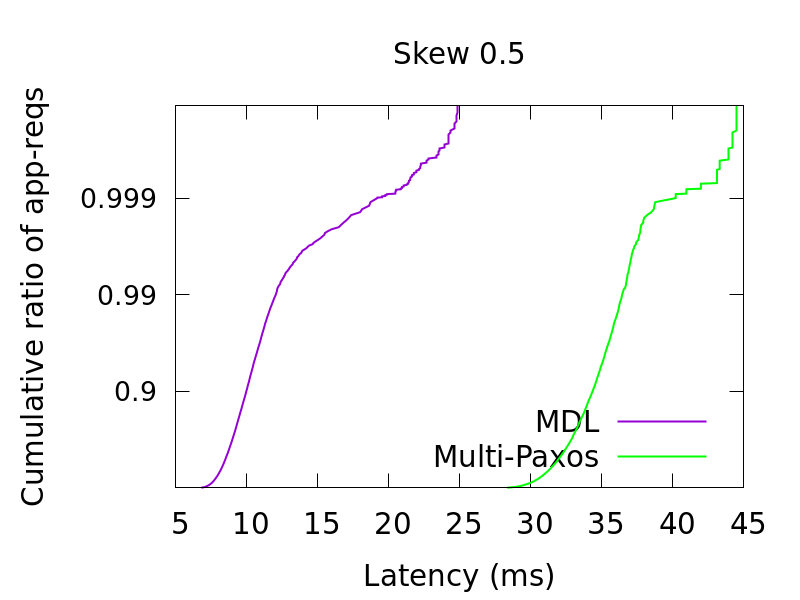
\includegraphics[scale=.2]{figs/old/9shards_fanout100_skew0.5_8client_CDF.png}
%   \label{fig:9shardsskew}
% }
% \subfloat[skew\xspace0.9]{
%   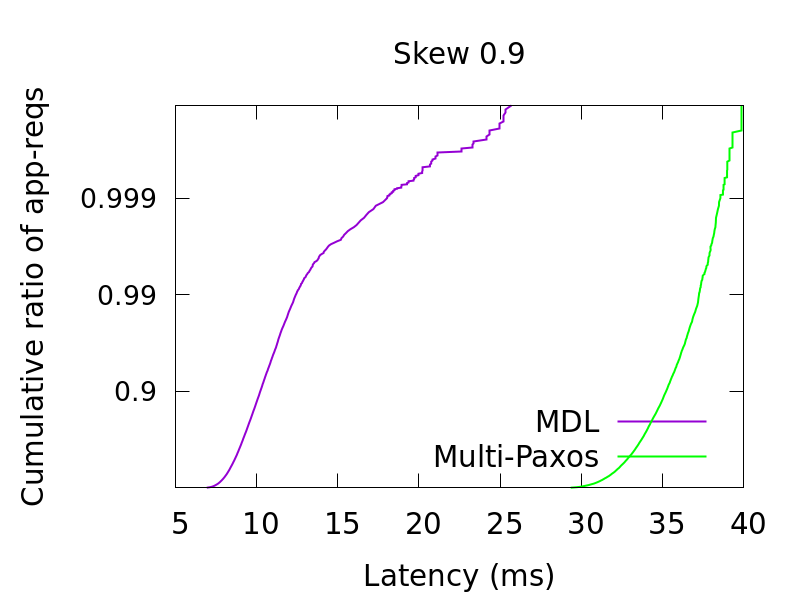
\includegraphics[scale=.2]{figs/old/9shards_fanout100_skew0.9_8client_CDF.png}
% }
% \subfloat[skew\xspace1.3]{
%   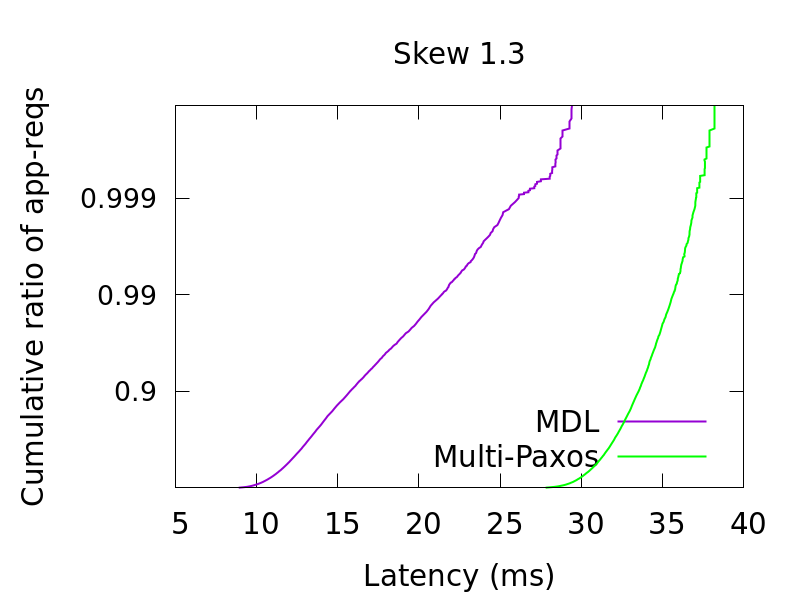
\includegraphics[scale=.2]{figs/old/9shards_fanout100_skew1.3_8client_CDF.png}
%   \label{fig:9shardsskewlast}
% }
% \caption{9 shard skew.}
% \end{figure*}

% %%%%%%%%%%%%%%%%%%%%%%%%%%%%%%%%%%%%%%%%%%%%%%%%%%%%%%%%%%%%%%%%%%%%%%%%%%%%%%%%%%%
% %%%%%%%%%%%%%%%%%%%%%%%%%%%%%%%%%%%%%%%%%%%%%%%%%%%%%%%%%%%%%%%%%%%%%%%%%%%%%%%%%%%
% %%%%%%%%%%%%%%%%%%%%%%%%%%%%%%%%%%%%%%%%%%%%%%%%%%%%%%%%%%%%%%%%%%%%%%%%%%%%%%%%%%%

% % \Crefrange{fig:3shardsskew}{fig:3shardsskewlast} and
% % ~\ref{fig:9shardsskew}--\ref{fig:9shardsskewlast} show various skew values for
% % the 3-shard and 9-shard configurations. 

% \Crefrange{fig:9shardsskew}{fig:9shardsskewlast} and
% show various skew values for
% the 9-shard configurations. 
% (Figures for a 3-shard configuration are similar and are omitted due to space constraints.)


% We generate keys according to a Zipfian
% distribution with varying skew values $\theta \in \{0.5, 0.9, 1.3\}$,
% and use a keyspace of size 1 million. We look at CDFs for application-level
% requests with fanout 100 issued by 8 concurrent clients.

% Increasingly higher skew approaches single shard performance, where \system's
% coordination is cheaper, as it does not include network latency, but experiences
% overload sooner.  Overall skew has little impact on end-to-end latency until a
% high skew value of 1.3, where the tail latency for application-level requests
% starts increasing at lower percentiles, by about 2x. We notice this degradation
% begin earlier at around skew 1.1 as well. We expect much of this is due to the
% high load on the leader responsible for highly contentious keys.

% \subsection{Single-Shard Optimization}
% We investigate the performance of a modification to the multi-dispatch protocol optimized for the single-shard setting, and compare it with the original multi-dispatch protocol as well as multi-paxos. The main modifications include removing coordination messages and removing the 2nd “ordering” round between leaders and replicas for all requests, as the first and only round replicates both a request as well as its index in the log. We keep the sequence numbers and buffer requests that arrive out-of-order wrt to their expected next sequence number.
% \begin{figure*}[tbp]
% \centering
% \subfloat[Fanout\xspace1]{
%   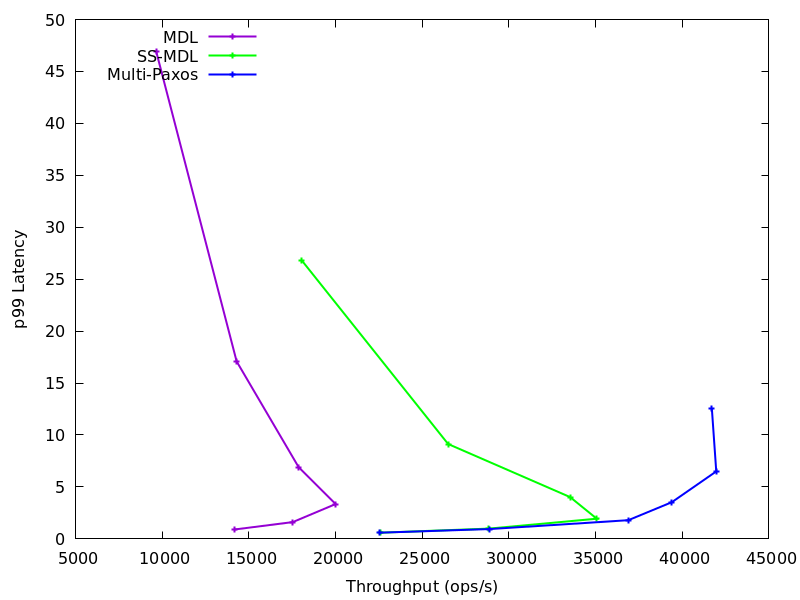
\includegraphics[scale=.2]{figs/ssa/ssa_f1.png}
%   \label{fig:SSA_f1}
% }
% \subfloat[Fanout\xspace10]{
%   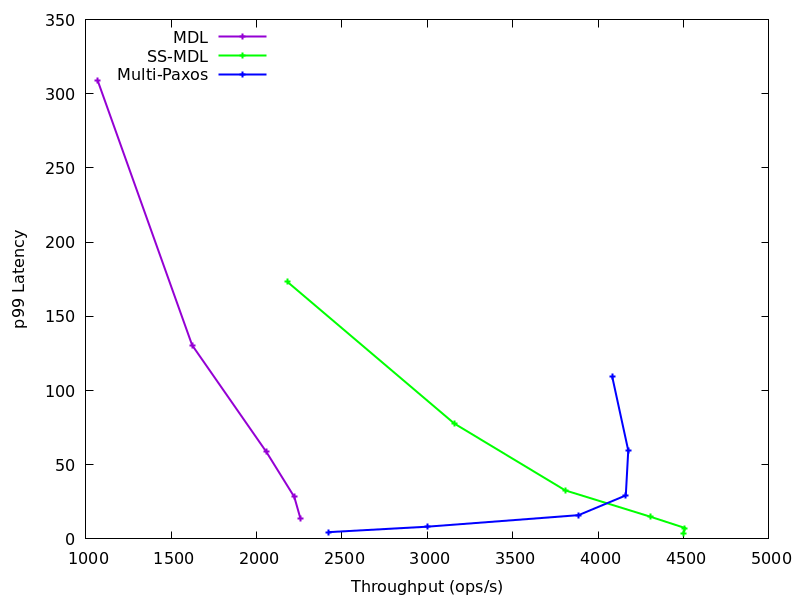
\includegraphics[scale=.2]{figs/ssa/ssa_f10.png}
%   \label{fig:SSA_f2}
% }
% \subfloat[Fanout\xspace100]{
%   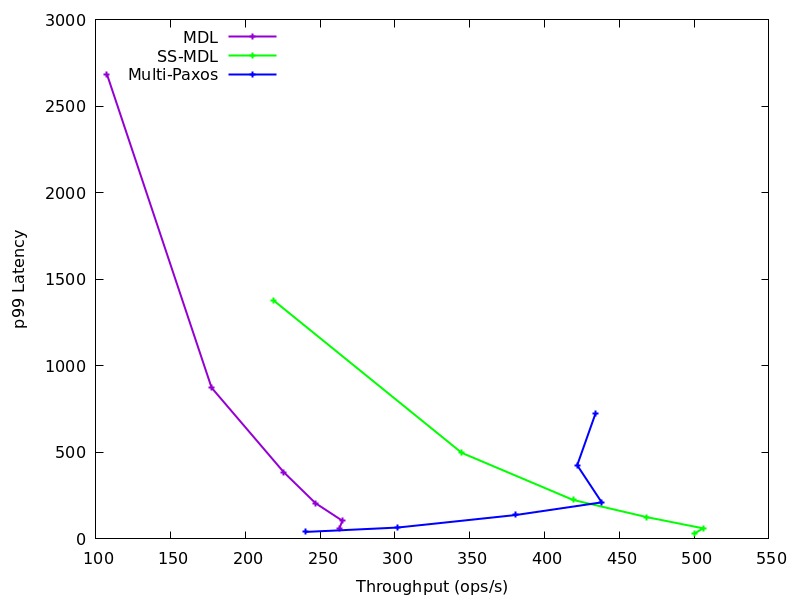
\includegraphics[scale=.2]{figs/ssa/ssa_f100.png}
%   \label{fig:SSA_f10}
% }
% \caption{Single-Shard Optimizations for fanouts 1, 10, 100}
% \label{fig:SSA}
% \end{figure*}

% As shown in figure ~\ref{fig:SSA}, without the optimizations, MDL cannot offer the same performance as SDL in the single-shard setting due to the overhead of coordination requests. With the optimizations, however, MDL can provide significantly higher throughput and lower latencies than SDL.

\begin{comment}
\subsection{MDL with Geo-rep in the Wide Area}
\label{sec:wide}
We show the e2e app. latency for varying inter-shard latency (which we call the wide area **this might be wrong terminology) and inter-replica latency (which we call geo-replication, also might be wrong terminology).

\subsection{Applications on MDL}
\label{sec:apps}

As described in prior sections, we built a tool to automatically transform applications built to interact with SDL backends to interact with MDL backends, maintaining external equivalence. In this section we select 3 representative applications, A1, A2, A3, and show that when transformed with our tool, all 3 see an improvement in e2e latency. We use DeathStar to benchmark the applications.

A1 is an application that ....

A2 is an application that ...

A3 is an application that ...

We expect transformed applications that have a large degree of data parallelism and are read heavy running on MDL backends to see the largest e2e latency improvements over their pre-transformed counterparts running on SDL backends.

Jeff is still looking for these applications at the moment -- it would be good to pick applications that are read heavy and some that are mixed. All should include varying degrees of data parallelism, to show how some improve after the transformation more than others.
\end{comment}
